\documentclass[a4paper]{article}

\usepackage[ampersand]{easylist}
\usepackage[nottoc,numbib]{tocbibind}
\usepackage{hyperref}
\usepackage{graphicx}
\usepackage{bbding}
\usepackage{listings}

\usepackage[colorinlistoftodos,prependcaption,textsize=tiny]{todonotes}
\newcommandx{\unsure}[2][1=]{\todo[linecolor=red,backgroundcolor=red!25,bordercolor=red,#1]{#2}}
\newcommandx{\change}[2][1=]{\todo[linecolor=blue,backgroundcolor=blue!25,bordercolor=blue,#1]{#2}}
\newcommandx{\info}[2][1=]{\todo[linecolor=OliveGreen,backgroundcolor=OliveGreen!25,bordercolor=OliveGreen,#1]{#2}}
\newcommandx{\improvement}[2][1=]{\todo[linecolor=Plum,backgroundcolor=Plum!25,bordercolor=Plum,#1]{#2}}
\newcommandx{\thiswillnotshow}[2][1=]{\todo[disable,#1]{#2}}

\title{\href{https://datsoftlyngby.github.io/soft2020fall/resources/8af56d7d-assignment-01.pdf}{Assingment} 1}
\author{Daniel Lindholm}
\date{October 15, 2020}

\begin{document}

\maketitle
\thispagestyle{empty}
\clearpage

\tableofcontents

\section{Task 2}
Produce a template (in LATEX, of course) that you can use in your bachelor
thesis

\subsection{Graphics}

\subsubsection{Image caption}
\begin{figure}[h!]
  \caption{My favorite duck image!}
  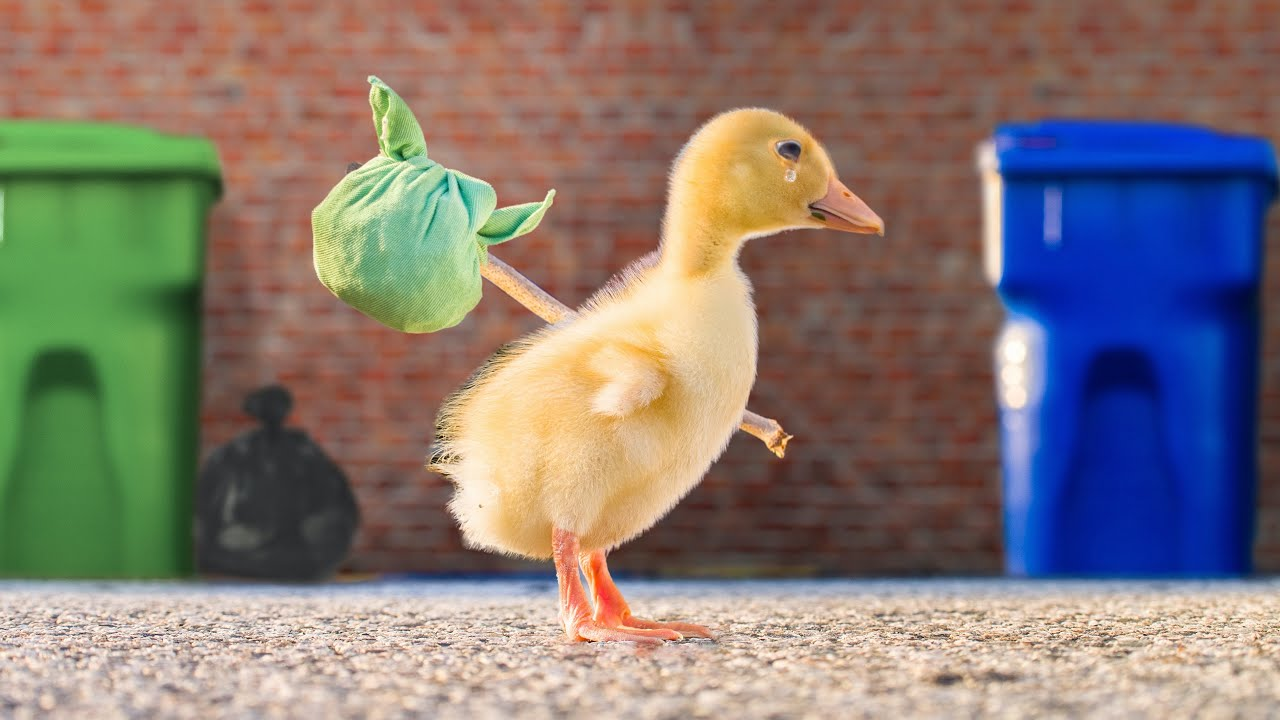
\includegraphics[width=0.5\textwidth]{duckz.jpg}
  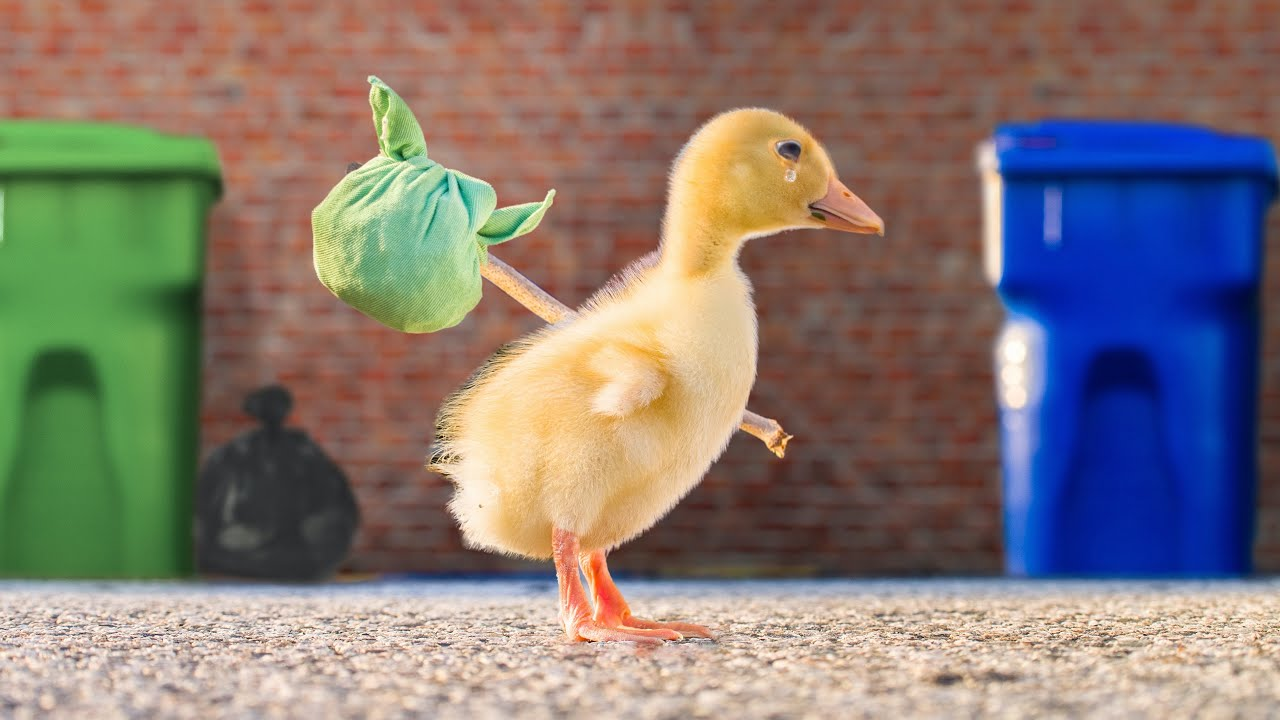
\includegraphics[width=0.5\textwidth]{duckz.jpg}
  \caption{My favorite duck image!}
\end{figure}

\begin{center}
  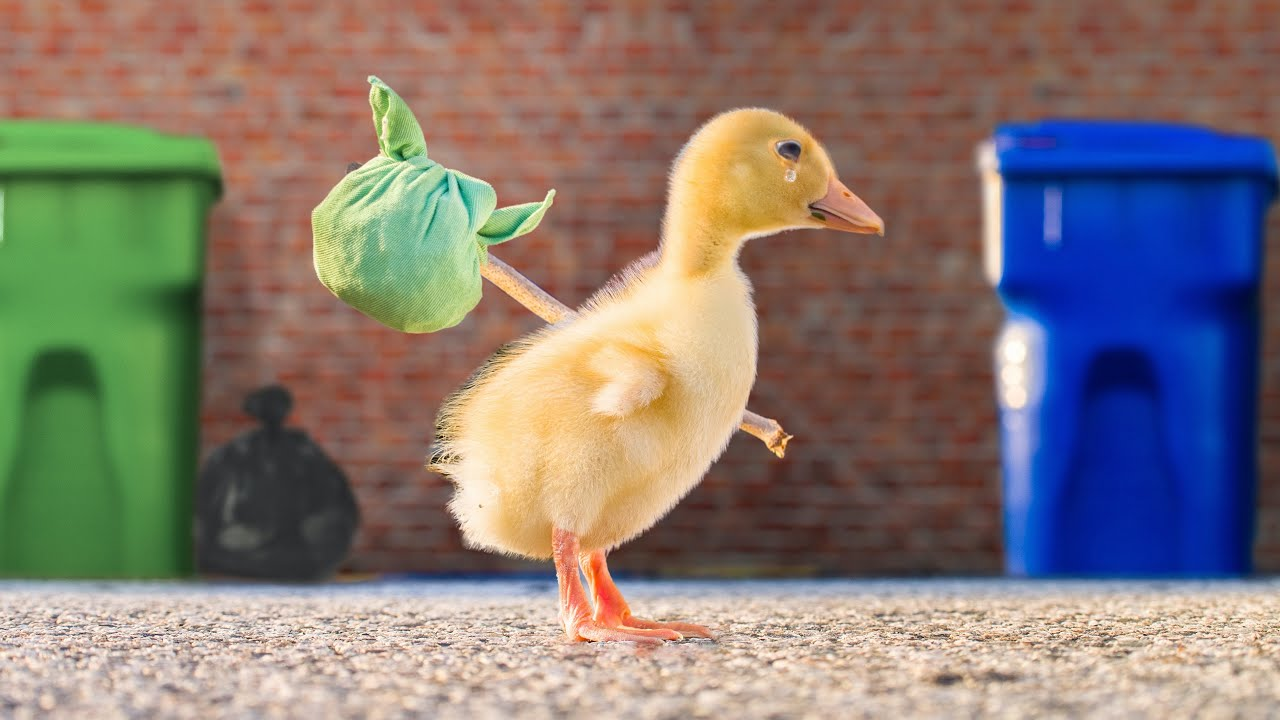
\includegraphics[width=0.5\textwidth]{duckz.jpg}
  \label{fig:duck}
\end{center}

Picture of duck can be found here: \ref{fig:duck}


\subsection{Lists}
\begin{itemize}
  \item Duck
  \item Chicken
  \item Jacob
\end{itemize}

\begin{enumerate}
  \item A
  \item B
  \item C
\end{enumerate}


\renewcommand{\labelitemi}{\Checkmark}
\begin{itemize}
  \item A
  \item B
  \item C
\end{itemize}

\subsection{Table with multiple columns}
\begin{center}
\begin{tabular}{ |c|c|c| } 
 \hline
 \multicolumn{2}{c}{cell1} & cell3 \\ 
 cell4 & cell5 & cell6 \\ 
 cell7 & cell8 & cell9 \\ 
 \hline
\end{tabular}
\end{center}

\subsection{Code listing}
\begin{lstlisting}
import numpy as np
    
def incmatrix(genl1,genl2):
    m = len(genl1)
    n = len(genl2)
    M = None #to become the incidence matrix
    VT = np.zeros((n*m,1), int)  #dummy variable
    
    #compute the bitwise xor matrix
    M1 = bitxormatrix(genl1)
    M2 = np.triu(bitxormatrix(genl2),1) 

    for i in range(m-1):
        for j in range(i+1, m):
            [r,c] = np.where(M2 == M1[i,j])
            for k in range(len(r)):
                VT[(i)*n + r[k]] = 1;
                VT[(i)*n + c[k]] = 1;
                VT[(j)*n + r[k]] = 1;
                VT[(j)*n + c[k]] = 1;
                
                if M is None:
                    M = np.copy(VT)
                else:
                    M = np.concatenate((M, VT), 1)
            
                VT = np.zeros((n*m,1), int)
    return M
\end{lstlisting}




\subsection{Todo}
lorem ipsum dolar summit1g.
\todo{Change this pliz}

\nocite{*}

\bibliographystyle{plain}
\bibliography{references}

\end{document}